\section{Heterogeneous computing}


异构计算的基本知识会在这里进行阐述。


$$\text{Processing Units} \begin{cases}
    \begin{rcases}
        \text{CPU} 
            \begin{cases}
                \text{Intel few-core CPU (Kaby Lake \textit{etc.})}\\
                \text{Intel many-core CPU (Xeon \textit{etc.})}\\
                \text{AMD}\\
                \text{\textit{etc.}}
            \end{cases} 
        \\
        \text{GPU} 
            \begin{cases}
                \text{Intel Integrated GPU}\\
                \begin{rcases} \text{NVIDIA (Titan \textit{etc.})} \end{rcases}  \text{Supported by CUDA}\\
                \text{AMD}\\
                \textit{etc.}
            \end{cases}
        \\
        \text{FPGA}
            \begin{cases}
                \text{Xilinx}\\
                \textit{etc.}
            \end{cases}
    \end{rcases} \text{Supported by OpenCL}
    \\
    \text{ASIC}
\end{cases}$$

OpenCL 是由非盈利性组织 Khronos Group 组织发布的针对异构设备进行并行化计算的一套开源的 API 以及程序语言。当年 Apple 为了让几大处理器厂商不会因为某一个给它供货导致市场被垄断,如果是其他电子厂商说这话可能 NVIDIA、 AMD 就笑一笑,但 Apple 说这话把他们硬是联合起来于 2008 年公开发布了一个异构计算的 convention,也就是我们用到的 OpenCL。

OpenCL 提供两种并行化的模式,包括\textbf{任务并行}以及\textbf{数据并行},目前针对 GPU 的引用,主要是以数据并行为主(因为 CUDA 实际上没办法做任务并行)。OpenCL API是按照 C API定义的,由 C 和 C++ 封装而成。使用OpenCL C语言编写的代码可以在支持OpenCL的设备上运行。OpenCL C是 C99 语言的子集,并适当地扩展到众多异构设备上执行数据并行代码的能力。

所谓异构设备,就是指底层硬件架构有较大不同的设备,比如 CPU 与 GPU,FPGA(可编程门阵列),CPU 中负责分支预测及跳转的控制单元和cache占据较大的面积,而 ALU(算术逻辑单元)占据的比重远远小于GPU中的ALU面积比重,换句话说,CPU强于控制,弱于计算,而GPU强于计算,弱于控制。

\begin{figure}[!htbp]
    \centering
    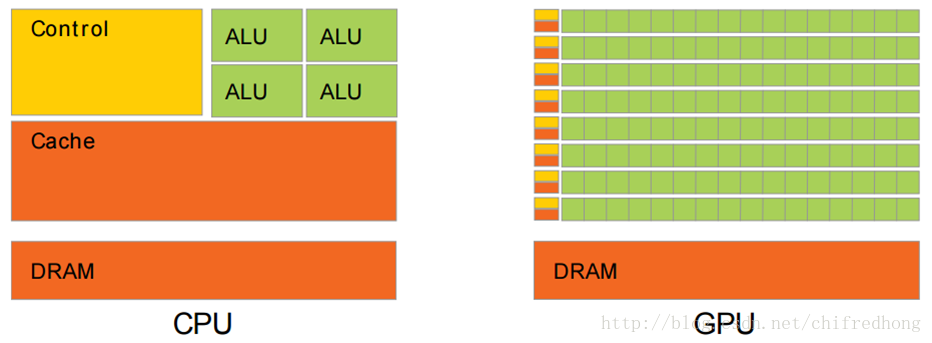
\includegraphics[width=.8\textwidth]{figure/CPU_GPU_structure.png} 
    \caption{CPU and GPU Structures} %caption是图片的标题
    % \label{img} 
\end{figure}
上图中,绿色部分是逻辑计算单元,红色的存储单元,橙黄色的是控制单元。

而FPGA近几年在深度学习、数据中心的部署,让它渐渐崭露头角。它的内部结构不像CPU和GPU那样把电路结构固化在芯片中,而是由LUT(查找表)、寄存器等基本器件构成,然后通过内部密集的互联线连接到IO。使用时,通过USB接口向设备传输一个二进制文件(位流),将其内部基本器件集合设置成针对某个应用的具体的电路结构。简单来讲,这相当于FPGA内部有数量及其庞大的开关,然后我们输入一股有规律的电流,将涉及到的开关拉高,并且暂时固定位置,而一旦开关都设置好以后,电路可以执行一定的功能。

\begin{figure}[!htbp]
    \centering
    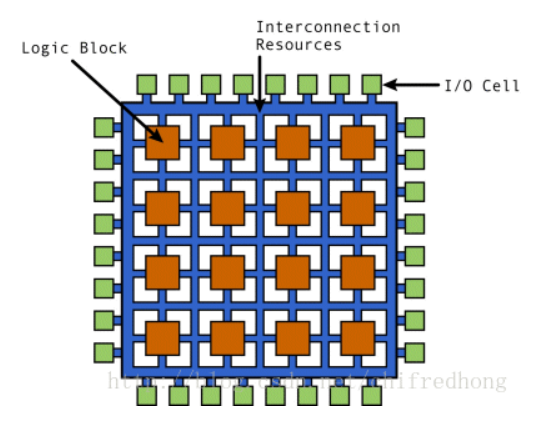
\includegraphics[width=.6\textwidth]{figure/FPGA_structure.png} 
    \caption{FPGA Structure} %caption是图片的标题
    % \label{img} 
\end{figure}

现在的主流的两大FPGA厂商Intel(本质上是Altera,被Intel收购了)和Xilinx,他们都提供了针对OpenCL标准开发的软件套件,目的就是避开传统FPGA开发中,使用硬件描述语言(verilog或VHDL)开发中周期长、流程复杂的缺点,使用高级语言(例如C语言)开发FPGA应用,降低了使用FPGA开发的门槛。
基本上,现在主流的异构计算架构都是主-从架构,主机通常是CPU,而从设备是GPU或FPGA,二者通过PCIe接口通信。

开发环境安装
OpenCL平台和OpenCL设备
一个opencl平台通常对应一个供应商。它负责为其设备提供opencl实现。例如,具有i7-4790 intel cpu的机器将会有一个opencl平台,大概命名为“intel opencl”,该平台将包括两个opencl设备:一个是intel cpu本身,另一个是intel hd graphics 4600 GPU。这个“intel opencl”平台正在为这两个设备提供opencl实现,并负责管理它们。
让我们再来一个例子,但这次是从Windows生态系统外面。运行os x的macbook和intel iris pro gpu和专用的geforce卡都将显示一个名为“apple”的opencl平台。两个gpus和cpu将显示为属于此平台的设备。这是因为“苹果”平台是为所有三种设备提供opencl实现的平台

但请记住:
1、opencl平台可以有一个或多个设备。
2、相同的设备可以具有来自不同供应商的一个或多个opencl实现。换句话说,opencl设备不仅可以属于一个平台。
3、该平台的opencl版本不一定与设备的opencl版本相同。

ICD和ICD loader
1、icd(可安装的客户端驱动程序),它是针对某个特定设备的专门的opencl实现,也就是opencl运行时。可以在amdocl.so/dll或intelopencl.so/dll这样的文件中找到它。它是指允许多个opencl平台共存的模型。它并不是核心功能,而是opencl的扩展。

2、icd loader(在opencl.dll / libopencl.so中):OpenCL Installable Client Driver (ICD) Loader是实现OpenCL应用程序与各硬件厂商提供的OpenCL驱动(platform)之间隔离的中间库。它用于管理同一系统中的多个icds

它与opencl应用程序相关联,并作为icd的占位符。
应用程序调用icd加载程序库导出的函数。然而,icd加载器根据所选的opencl平台决定要重定向到哪个icd。
icd加载机制是必需的,因为供应商的opencl实现通常只支持该供应商的硬件,但您可能希望在同一个opencl应用程序中使用来自不同供应商的多个设备。

% icd只是一个可选的opencl扩展,标识符是cl_khr_icd。当你安装了某个厂商的SDK,就会在操作系统的注册表上添加相应的注册表项。opencl icd loader允许应用程序调用clIcdGetPlatformIDsKHR函数获取所有已经安装的平台的列表,从中选择一个平台,并将opencl api调用发送到底层实现。 khronos注册表中提供了icd加载程序库的源代码https://github.com/KhronosGroup/OpenCL-ICD-Loader。

注意,一台机器可以有几个opencl平台,每个平台都有自己的驱动程序和opencl版本,总是只有一个icd加载程序。 icd加载器充当所有安装的opencl平台的主管,并为所有opencl调用提供了唯一的入口点。基于平台ID,它将opencl主机调用分配到正确的驱动程序。

这样你就可以编译icd(windows上的opencl.dll或者linux上的libopencl.so),而不是直接给所有可能的驱动程序编译。在运行时,opencl应用程序将搜索icd并加载它。 icd依次在注册表(Windows)或特殊目录(linux)中查找注册的opencl驱动程序。您的软件的每个opencl调用将由icd解决,这将进一步调度请求到所选的opencl平台。

% ICD loader在Windows上如何枚举Vendors?
% 在Windows上,和厂商想关的库文件是设定在注册表中的。ICD loader会扫描注册表项HKEY_LOCAL_MACHINE\SOFTWARE\Khronos\OpenCL\Vendors的值,当DWORD中的每个值都为0时,ICD loader打开由名称指定的动态链接库,使用LoadLibraryA的值。例如,如果注册表[HKEY_LOCAL_MACHINE\SOFTWARE\Khronos\OpenCL\Vendors]包含下列值"c:\\vendor a\\vndra_ocl.dll"=dword:00000000,那么ICD loader将打开"c:\vendor a\vndra_ocl.dll"库文件
% 添加Vendors
% 在成功加载了一个厂商ICD库后,ICD loader会从库文件中查询下列函数clIcdGetPlatformIDsKHR, clGetPlatformInfo, 和clGetExtensionFunctionAddress.如果其中任意一个函数不存在,则ICD loader会关闭并且忽略这个厂商的ICD库。
% 接下来,ICD loader查询可用的ICD-enable 平台,这个过程使用库中的clIcdGetPlatformIDsKHR函数。 对于每一种平台上,ICD加载器查询 平台的扩展字符串来验证cl_khr_icd的 支持,然后使用clGetPlatformInfo函数查询平台的厂商ICD扩展后缀 ,函数使用CL_PLATFORM_ICD_SUFFIX_KHR参数, 如果其中任何一个步骤失败,ICD loader将忽略 厂商ICD并继续到下一个。

% 配置VS2012 OpenCL开发环境:
% AMD GPU平台
% 说明,以下的是针对Win7 AMD APP SDK 2.9版本的OpenCL开发环境搭建

% 1、环境变量
% 安装完AMD APP SDK 2.9后,系统会自动添加
%  \emph{\$(AMDAPPSDKROOT)} 环境变量,值是安装时指定的路径。
% 2、添加头文件
% 在项目->属性->配置属性->C/C++->附加包含目录中添加
% $(AMDAPPSDKROOT)/include
% (C:\Users\server\AMD APP SDK\2.9-1\include和C:\Users\server\AMD APP SDK\2.9-1\include\SDKUtil可添可不添)
% 3、添加库目录
% 在项目->属性->配置属性->链接器->附加库目录中添加
% $(AMDAPPSDKROOT)\lib\x86(win32项目配置)或:\$(AMDAPPSDKROOT)\lib\x86_64(x64项目配置)
% 4、添加库输入
% 使用AMD SDK平台时,需要配置OpenCL.lib文件,具体方法:项目->属性->配置属性->连接器->输入->附件依赖库->编辑,添加OpenCL.lib
% 5、主机代码
% 在主机程序代码中添加#include <CL/cl.h>

% Intel FPGA平台
% 说明,以下的是针对Win7 Quartus 14.0版本的OpenCL开发环境搭建
% 安装顺序:Intel FPGA Design Software -> Intel FPGA SDK for OpenCL->FPGA PCIe 驱动 -> Visual Studio 2012 -> CodeXL

% Intel FPGA Design Software 和Intel FPGA SDK for OpenCL下载地址
% 注意:Intel FPGA SDK for OpenCL需要license,不然无法编译OpenCL内核设计文件。同时,把相应开发板的BSP(板级开发包),复制到Intel FPGA Design Software 的目录下。BSP里面包含FPGA板子board_env.xml描述文件,这个文件指出设备的名字、链接器输入库的名字以及相应驱动程序所在目录等信息。

% 1、环境变量
% 安装完Intel FPGA Design Software 和Intel FPGA SDK for OpenCL后,环境变量中会自动添加 ALTERAOCLSDKROOT,其值为相应平台安装后的路径。另外,还需要添加AOCL_BOARD_PACKAGE_ROOT 这个环境变量,它的值为相应BSP的路径

% 2、设置解决方案的配置
% 因为 Intel 的 OpenCL 只支持 64 位的系统,所以在这里没有了 32位和 64 位之分,项目->属性->活动解决方案平台->新建->键入或选择新平台,选择 x64 作为当前解决方案的平台。
% 3、添加头文件
% 在项目->属性->配置属性->C/C++->附加包含目录中添加
% $(ALTERAOCLSDKROOT)\host\include
% 4、添加库目录
% 在项目->属性->配置属性->链接器->附加库目录中添加
% $(ALTERAOCLSDKROOT)\host\windows64\lib 和$(AOCL_BOARD_PACKAGE_ROOT)\de5net\windows64\lib
% 5、添加库输入
% 项目->属性->配置属性->连接器->输入->附件依赖库->编辑,添加

% alterahalmmd.lib
% terasic_apb_14_0_mmd.lib
% alteracl.lib
% acl_emulator_kernel_rt.lib
% pkg_editor.lib
% libelf.lib
% acl_hostxml.lib
% 1
% 2
% 3
% 4
% 5
% 6
% 7
% 至此,面向OpenCL的软件开发平台安装完成~
% ————————————————
% 版权声明:本文为CSDN博主「chifredhong」的原创文章,遵循 CC 4.0 BY-SA 版权协议,转载请附上原文出处链接及本声明。
% 原文链接:https://blog.csdn.net/chifredhong/article/details/73931017


\cite{OpenCL浅析}